\documentclass[]{article}
\usepackage{proceed2e}
\usepackage{enumerate}
\usepackage{algpseudocode}
\usepackage[ruled]{algorithm}
\usepackage{url}
\usepackage{framed}
\usepackage{amsfonts,amsmath,amsthm,amssymb}
\usepackage{graphicx}
\usepackage{url}
\usepackage{color}
\usepackage[round]{natbib}
\usepackage{comment}

\def\citeapos#1{\citeauthor{#1}'s (\citeyear{#1})}

\newcommand {\mean} {\ensuremath {\mathop{\mathrm{mean}}}}
\newcommand {\median} {\ensuremath {\mathop{\mathrm{median}}}}
\newcommand {\N} {\ensuremath {\mathcal{N}}}
\newcommand {\IE} {\ensuremath {\mathbb{E}}}
\newcommand {\cov} {\ensuremath {\mathop{\mathrm{cov}}}}
\newcommand {\BEL} {\ensuremath {\mathop{\mathrm{BEL}}}}

\newcommand {\term}[1] {\textbf{#1}}
\newcommand {\note}[1] {\textcolor{red}{[[#1]]}}
\newcommand {\Evidence} {\mathcal{E}}
\newcommand {\R} {\mathbb{R}}
\newcommand {\maps} {\colon}
\newcommand {\given} {\mid} %{\mathrel{|}}
\newcommand {\sample} {\sim}
\newcommand {\iid} {\stackrel{\rm iid}{\sample}}
\newcommand {\Nat} {\mathbb{N}}
\DeclareMathOperator*{\argmax}{argmax}

\newtheorem{thm}{Theorem}
\newtheorem{dfn}[thm]{Definition}
\newtheorem{lmm}[thm]{Lemma}
\newtheorem{crl}[thm]{Corollary}
\newtheorem{example}{Example}

\newcommand{\secref}[1]{Section~\ref{#1}}
\newcommand{\secrefs}[2]{Sections~\ref{#1} and~\ref{#2}}
\newcommand{\figref}[1]{Figure~\ref{#1}}
\renewcommand{\eqref}[1]{Equation~(\ref{#1})}
\newcommand{\eqrefs}[2]{Equations~(\ref{#1}) and~(\ref{#2})}
\newcommand{\thmref}[1]{Theorem~\ref{#1}}
\newcommand{\dfnref}[1]{Definition~\ref{#1}}
\newcommand{\exampleref}[1]{Example~\ref{#1}}

\excludecomment{hiddenproof}

\title{Selecting Computations: Theory and Applications} 

\author{}
%\author{ {\bf Nicholas Hay} and {\bf Stuart Russell} \\   
%Computer Science Division \\  
%University of California\\ 
%Berkeley, CA 94720 \\ 
%\And 
%{\bf Solomon Eyal Shimony} and {\bf David Tolpin}  \\ 
%Department of Computer Science \\ 
%Ben-Gurion University of the Negev\\
%Beer Sheva, Israel
%} 
 

\begin{document}

\maketitle 

\begin{abstract}
Sequential decision problems are often approximately solvable by
simulating possible future action sequences.  {\em Metalevel} decision
procedures have been developed for selecting {\em which} action
sequences to simulate, based on estimating the expected
improvement in decision quality that would result from any particular
simulation; an example is the recent work on using bandit algorithms
to control Monte Carlo tree search in the
game of Go.  In this paper we develop a theoretical basis for
metalevel decisions in the statistical framework of Bayesian {\em selection problems}, 
arguing (as others have done) that this is more appropriate than the bandit
framework.  We derive a number of basic results applicable to 
Monte Carlo selection problems, including the first finite sampling
bounds for optimal policies in certain cases; we also provide a simple
counterexample to the intuitive conjecture that an optimal policy will
necessarily reach a decision in all cases.  We then derive heuristic
approximations in both Bayesian and distribution-free settings and
demonstrate their superiority to bandit-based heuristics in one-shot
decision problems and in Go.
\end{abstract}


\section{Introduction}

The broad family of sequential decision problems includes
combinatorial search problems, game playing, robotic path planning,
model-predictive control problems, Markov decision processes (MDP), whether fully or
partially observable, and a huge range of applications. In almost all
realistic instances, exact solution is intractable and approximate
methods are sought. Perhaps the most popular approach is to simulate
a limited number of possible future action sequences, 
in order to find a move in the current state that is (hopefully)
near-optimal. One of the most successful
examples of this approach are sampling algorithms for
playing the game of Go \citep{Gelly.mogo} based on the upper-confidence bound (UCB)
method \citep{Kocsis+Szepesvari:2006}. This paper examines the issue of sampling for move selection from
first principles, by defining an appropriate meta-level MDP and formally
analyzing some of its properties. Although
the meta-level MDP is also intractable, approximation schemes based on
provable value of information bounds for this problem are presented. 
These lead to practical sampling schemes that
are promising: they out-perform the UCB-based schemes,
as indicated by empirical results on both ``flat'' selection and
game-playing in Go.

As selection is extremely general \citep{TolpinShimony:2012}, we focus on the adversarial
game-playing domain as an example for clarity.
A typical game-playing algorithm explores a tree or graph of action sequences
with some limit on depth, using pruning methods to avoid irrelevant
subtrees; based on what it finds in the explored portion of the state space, the algorithm
then selects a move. This exploration is repeated after observing the move
made by the opponent (whether or not information from previous explorations
is reused is discussed in Section \ref{sec:control-redistribution}).

Clearly, it is desirable to select the best possible move using the
least possible amount of exploration. For a given amount of
exploration, decision quality can be improved by directing exploration
towards those actions sequences whose outcomes are helpful in selecting
a good move. Thus, the {\em metalevel} decision problem is to choose
what future action sequences to explore (or, more generally, what
deliberative computations to do), while the {\em object-level}
decision problem is to choose an action to execute in the real world.

That the metalevel decision problem can itself be formulated and
solved decision-theoretically was noted by \citet{Matheson:1968},
borrowing directly from the related concept of {\em information value
  theory}~\citep{Howard:1966}. In essence, computations can be
selected according to the expected improvement in decision quality
resulting from their execution. I. J.~\citet{Good:1968} independently
proposed using this idea to control search in chess, and later defined
``Type II rationality'' to refer to agents that optimally solve the
metalevel decision problem before acting. As interest in probabilistic
and decision-theoretic approaches in AI grew during the 1980s, several
authors explored these ideas further~\citep{Dean+Boddy:1988,Doyle:1988,Fehling+Breese:1988,Horvitz:1987b}.
Work by
\citet{Russell+Wefald:1988a,Russell+Wefald:1991a,Russell+Wefald:1991b}
formulated the metalevel sequential decision problem, employing an
explicit model of the results of computational actions, and applied
this to the control of game-playing search in Othello with encouraging
results.

An independent thread of research on metalevel control began with work
by \citet{Kocsis+Szepesvari:2006} on the UCT algorithm, which operates
in the context of {\em Monte Carlo tree search} (MCTS) algorithms.
In MCTS, each computation takes the form
of a simulating a randomized sequence of actions leading from a leaf of the
current tree to a terminal state. UCT is primarily a method for
selecting a leaf from which to conduct the next simulation, and
forms the core of the successful \textsc{MoGo} algorithm for Go 
playing \citep{Gelly+Silver:2011}.  The UCT algorithm is
based on the the theory of bandit problems \citep{Berry+Fristedt:1985} and the near-optimal
UCB1 bandit algorithm \citep{Auer+et+al:2002}. UCT applies
UCB1 recursively to select actions to perform within simulations.

It is natural to consider whether the two independent threads are
consistent; for example, are bandit algorithms such as UCB1 approximate
solutions to some particular case of the metalevel decision problem
defined by Russell and Wefald? The answer, perhaps surprisingly, is no.
The essential difference is that, in bandit problems, every trial involves
executing a real object-level action with real costs, whereas in the metareasoning
problem the trials are {\em simulations} whose cost is usually independent of the
utility of the action being simulated. 
Hence, in UCT, bandit algorithms are applied to problems that are not bandit problems.

One consequence of the mismatch is that bandit policies are
inappropriately biased away from exploring actions whose current
utility estimates are low.  Another consequence is the absence of any
notion of ``stopping'' in bandit algorithms, which are designed for
infinite sequences of trials.  A metalevel policy needs to decide
when to stop deliberating and execute a real action.

Analyzing the metalevel problem within an appropriate theoretical
framework ought to lead to more effective algorithms than those
obtained within the bandit framework.  For Monte Carlo computations,
in which samples are gathered to estimate the utilities of actions,
the metalevel decision problem is an instance of the {\em selection
problem} studied in statistics~\citep{Bechhofer:1954,Swisher+et+al:2003}.  Despite
recent work by \citet{Frazier+Powell:2010} and \citet{TolpinShimony:2012}, the theory of selection
problems is less well understood than that of bandit problems.
Accordingly, we present in \secrefs{sec:optimal}{sec:context}
a number of results concerning optimal policies for the general case
and for specific sampling distributions. In particular, we give finite
bounds on the number of samples collected by optimal policies for
Bernoulli and Gaussian distributions. We also provide a simple
counterexample to the intuitive conjecture that an optimal policy
should not spend more on deciding than the decision is worth; in fact,
it is possible for an optimal policy to compute forever. We also show
by a simple counterexample that optimal {\em index
policies}~\citep{Gittins:1989} do not necessarily exist for selection
problems.

Motivated by this theoretical analysis, we propose in \secrefs{approx-bayesian-section}{approx-nonbayesian-section}
two families of heuristic approximations, one for the
Bayesian case and one for the distribution-free setting.
We show empirically that these rules give better performance than UCB1 on 
a wide range of standard (non-sequential) selection problems.
\secref{mcts-section} shows similar results for the case of guiding Monte Carlo tree search
in the game of Go.


%% [[frazier]]

[[bubeck et al; see Shimony's earlier related work section]]

[[simulation community, Swisher survey; explain focus on probability of error]]

[[budgeted learning (incl the hardness and approx policy paper)]]


\section{On optimal policies for selection}\label{sec:optimal}

%% \section{On optimal policies for selection}

%% Define selection problem and metalevel MDP representation.

%% \note{Unsure about terminology here: selection problems, sampling problems, 
%% metalevel probability model, metalevel decision problem (conflicts with Markov decision process?).}

%% ============================
%% \subsection{Selection problems}
%% ============================

%% \note{Formal definition of selection problems and the metalevel MDP with cost per sample (time value); also mention budgeted learning.}

In a \term{selection problem} the decision maker is faced with the choice between
alternative actions.  To make this choice, they may gather evidence about the
utility of each of these alternative, at some cost.  The objective is to maximize
the expected utility of the final action selected, less the cost of computation.

%% This problem has been studied in a number of related forms.  \note{Here}

%% The Bayesian ranking and selection problem \citep{Swisher+et+al:2003} is an important
%% special case where the computations performed are samples.

%%What the decision maker can know and what they can find out is formalized in:

\begin{dfn} \label{dfn:metalevel-model}
	A \term{metalevel probability model} is a tuple $M=(U_1,\dots,U_k,\Evidence)$ 
	consisting of jointly distributed random variables:
	\begin{itemize}
		\item Real random variables $U_1,\dots,U_k$, where $U_i$ is the utility of performing action~$i$ (called ``arms" in the bandit setting), and
		\item A countable set $\Evidence$ of random variables, each variable $E\in\Evidence$ being 
		      a computation that can be performed and whose value is the result of that computation.
	\end{itemize}
\end{dfn}
%% Not actually true that we necessarily define this with U's as roots:  in sampling models they are naturally /leaves/.

A metalevel probability model, when combined with a cost $c>0$ of computation,%
\footnote{The assumption of a fixed cost of computation is a simplification; 
	precise conditions for its validity are given by \citep{Harada:1997}.} 
defines a metalevel decision problem: what is the optimal strategy with which to choose a sequence 
of computations $E\in\Evidence$ to observe in order to maximize the expected utility 
of the action finally taken less the cost of computation?  Intuitively, 
this strategy should observe the variables which give the most evidence relevant
to deciding which action to perform, stopping when the cost of computation 
outweighs the benefit gained.

\begin{example}[Bernoulli sampling]\label{example:bernoulli}
%% One simple metalevel probability model is used as a model of the results of simulations \citep{someone}.
In the \term{Bernoulli metalevel probability model},
each action will either succeed or not $U_i\in\{0,1\}$, with an unknown latent frequency of success $\Theta_i$, 
and stochastic simulations of possible consequences $E_{ij}$ can be performed:
\begin{align*}
	\Theta_i &\iid {\rm Uniform}[0,1]                      &&\quad\text{for $i=1,\dots,k$}\\
	U_i \given \Theta_i &\sample {\rm Bernoulli}(\Theta_i) &&\quad\text{for $i=1,\dots,k$}\\
	E_{ij} \given \Theta_i &\iid {\rm Bernoulli}(\Theta_i) &&\quad\text{for $i=1,\dots,k$ and $j=1,\dots$}
\end{align*}

The \term{one-action Bernoulli metalevel probability model} has $k=2$,
$\Theta_1=m\in[0,1]$ a constant, and $\Theta_2\sample{\rm Uniform}[0,1]$.
\end{example}

%% Bounedness assumption
For simplicity, in the below we'll assume the utilities $U_i$ are bounded and so, 
without loss of generality, lie in $[0,1]$.  

To formalize this problem, we use the theory of Markov Decision Processes (MDPs; 
see, for example, \citet{Puterman:1994}):

\begin{dfn}
A (countable state, undiscounted) \term{Markov Decision Process} (MDP) is a tuple $M=(S,s_0,A_s,T,R)$ where:
	$S$ is a countable set of states,
	$s_0\in S$ is the fixed initial state,
	$A_s$ is a countable set of actions available in state $s\in S$,
	$T(s,a,s')$ is the transition distribution 
	giving the probability of transitioning from a state $s\in S$ to a state $s'\in S$ after performing action $a\in A_s$,
	and $R(s,a,s')$ is the expected reward received when transitioning from $s\in S$ to $s'\in S$ after performing action $a\in A_s$.
\end{dfn}

\begin{dfn}\label{dfn:metalevel-mdp}
	Given a metalevel probability model%
		\footnote{Definition~\ref{dfn:metalevel-model} made no assumption about the computational result
			variables $E_i\in\Evidence$, but for simplicity in the following we'll assume that
			each $E_i$ takes one of a countable set of values.  Without loss of generality, 
			we'll further assume the domains of the computational variables $E\in\Evidence$ are disjoint.}
	$M=(U_1,\dots,U_k,\Evidence)$ and
	a cost of computation $c>0$, a corresponding \term{metalevel decision problem}
	is any MDP $M=(S,s_0,A_s,T,R)$ \begin{align*}
		S &= \{\bot\}\cup\{\langle e_1\dots, e_n \rangle : e_i\in E_i \text{ for all $i$,} \\
								& \qquad\qquad \text{for finite $n\ge0$ and distinct $E_i\in\Evidence$}\} \\
		s_0 &= \langle \rangle \\
		A_s &= \{\bot\}\cup\Evidence_s \\
	%
	\intertext{where $\bot\in S$ is the unique terminal state,
	where $\Evidence_s\subseteq\Evidence$ is a potentially state-dependent subset of allowed computations,
	and when given any $s=\langle e_1, \dots, e_n \rangle\in S$,
	computational action $E\in\Evidence$, 
	and $s'= \langle e_1, \dots, e_n, e \rangle\in S$ where $e\in E$, we have:}
	%
		T(s,E,s') &= P(E=e \given E_1=e_1,\dots,E_n=e_n) \\
		T(s,\bot,\bot) &= 1 \\
		R(s,E,s') &= -c \\
		R(s,\bot,\bot) &= \max_i \mu_i(s) % \max_i \IE[U_i \given E_1=e_1,\dots,E_n=e_n]
	\end{align*}		
	and where $\mu_i(s) = \IE[U_i \given E_1=e_1,\dots,E_n=e_n]$.
\end{dfn}



One can optionally add an external constraint on the number of computational actions, or their total cost,
in the form of a deadline (called a budget henceforth).  This bridges with the related area of budgeted learning \citep{Madani+et+al:2004}.
Although this feature is not formalized in the MDP, it can be added by including either time or past total cost 
as part of the state.

\begin{example}[Bernoulli sampling]\label{example:bernoulli2}
In the Bernoulli metalevel probability model (\exampleref{example:bernoulli}),
note that: 
\begin{align}
	\Theta_i \given E_{i1},\dots,E_{in_i} &\sim {\rm Beta}(s_i+1, f_i+1)  \label{eq:bernoulli1}\\
	E_{i(n_i+1)} \given E_{i1},\dots,E_{in_i} &\sim {\rm Bernoulli}\left(\frac{s_i+1}{n_i+2}\right) \label{eq:bernoulli2} \\
	\IE[U_i \given E_{i1},\dots,E_{in_i}] &= (s_i+1)/(n_i+2) \label{eq:bernoulli3}
\end{align}
by standard properties of these distributions, where $s_i=\sum_{j=1}^{n_i} E_{in_i}$
is the number of simulated successes of action $i$, and $f_i=n_i-s_i$ the failures.  By \eqref{eq:bernoulli1}, 
the state space is the set of all $k$ pairs $(s_i,f_i)$, \eqrefs{eq:bernoulli2}{eq:bernoulli3}
suffice to give the transition probabilities and terminal rewards, respectively.
The one-action Bernoulli case is similar, requiring only the two dimensional 
space $(s,f)$ giving the posterior over $\Theta_2$.
\end{example}


Given a metalevel decision problem $M=(S,s_0,A_s,T,R)$ one defines policies and 
value functions as in all MDPs.  A (deterministic, stationary) \term{metalevel policy} 
$\pi$ is a function mapping states $s\in S$ to actions to take in that state $\pi(s)\in A_s$.	

The \term{value function} for a policy $\pi$ gives the expected total reward
received under that policy starting from a given state $s\in S$, and the \term{Q-function}
does the state when starting in a state $s\in S$ and taking a given action $a\in A_s$: 
\[
	V^\pi_M(s) = \IE^\pi_M\left[ \sum_{i=0}^N R(S_i,\pi(S_i),S_{i+1}) \given S_0 = s\right]	\label{eq:value-fn}\\
%%	Q^\pi_M(s,a) &= \IE^\pi_M\left[ \sum_{i=0}^N R(S_i,\pi(S_i),S_{i+1}) \given S_0 = s, A_0 = a\right] \label{eq:qvalue-fn}
\]
where $N\in[0,\infty]$ is the random time the MDP is terminated, i.e.,
the unique time where $\pi(S_N)=\bot$%
\footnote{Whenever $N<\infty$, $S_{N+1}=\bot$ the unique terminal state.
Instead of having a random termination time, one can equivalently make
the state $\bot$ absorbing with zero reward on all transitions.}, 
and similarly for the Q-function $Q^\pi_M(s,a)$.

As usual, an \term{optimal policy} $\pi^*$, when it exists, is one which maximises 
the value from every state $s\in S$, i.e., if we define for each $s\in S$
\[
	V^*_M(s)   = \sup_\pi V^\pi_M(s),
%%	Q^*_M(s,a) &= \sup_\pi Q^*_M(s,a),
\]
then the optimal policy $\pi^*$ satisfies $V^{\pi^*}_M(s) = V^*_M(s)$
for all $s\in S$, where we break ties towards stopping $\bot$.
%% and by standard results, $\pi^*(s) \in \argmax_{a\in A_s} Q^*_M(s,a)$, where 

The optimal policy must balance the cost of computations with the improved decision
quality that results.  This is made clear by giving by expressing the value function:

\begin{thm}\label{thm:value-of-computation}
	The value function of a metalevel decision process $M=(S,s_0,A_s,T,R)$ is of the form
	\[
		V^\pi_M(s) = \IE^\pi_M[ -c\,N + \max_i \mu_i(S_N) \given S_0=s]
	\]
	where the random variable $N$ denotes the total number of computations performed,
	and similarly for $Q^\pi_M(s,a)$.
\end{thm}

\begin{proof}
	Follows immediately from \eqref{eq:value-fn} and the definition of the
	reward function in \dfnref{dfn:metalevel-mdp}.
\end{proof}

In many problems, including the Bernoulli sampling model of \exampleref{example:bernoulli2},
the state space is infinite.  Does this preclude solving for the optimal policy?  Can 
infinitely many computations be performed?

There is in full generality an upper bound on the \emph{expected} number of computations
a policy performs:

\begin{thm}\label{thm:bounded-expected-computations}
	The optimal policy $\pi^*$'s expected number of computations is bounded by the 
	perfect value of information \citep{Howard:1966} times the inverse cost $1/c$:
	\[
		\IE^{\pi^*}[N\given S_0=s] \le \frac{1}{c} \left(\IE[\max_i U_i\given S_0=s] - \max_i \mu_i(s)\right).
	\]
	Further, any policy $\pi$ with infinite expected number of computations 
	$\IE^\pi[N]=\infty$ has negative infinite value, so in particular the optimal
	policy stops with probability 1.
\end{thm}

\begin{proof}
	The first follows as in state $s$ the optimal policy has value at least that
	of stopping immediately $\max_i \mu_i(s)$, and as $\IE \max_i\mu_i(S_N) \le \IE \max_i U_i$ by Jensen's inequality.
	The second follows from \thmref{thm:value-of-computation} as $c>0$.
\end{proof}

However, although the \emph{expected} number of computations is always bounded,
there are important cases in which the \emph{actual} number is not, such as
the following example inspired by the sequential probability ratio test \citep{Wald+1945}:

\begin{example}\label{example:sprt}
Consider the Bernoulli sampling model for two actions but with different priors:
	$\Theta_1=1/2$,
	and $\Theta_2$ is $1/3$ or $2/3$ with equal probability.
%
Simulating action 1 gains nothing, and after $(s,f)$ simulated successes and failures of action 2
the posterior odds is
\[
	\frac{P(\Theta_2=2/3\given s,f)}{P(\Theta_2=1/3\given s,f)} = \frac{(2/3)^s(1/3)^f}{(1/3)^s(2/3)^f}= 2^{s-f}.
\]
Note that these odds completely specify the posterior distribution of $\Theta_2$,
and thus the distribution of the utility and all future computations.  Thus, whether
it is optimal to continue is a function only of this posterior odds, and thus $s-f$.
%% In particular,
%% note that after equal numbers of successes and failures, $s-f=0$ and so the posterior 
%% distribution over $\Theta_2$ is equal to the prior.
For sufficiently low cost, the 
optimal policy samples when $s-f$ equals $-1$, $0$, and $1$.  But with probability
$1/3$, a state with $s-f=0$ transitions to another state $s-f=0$ after two samples, 
giving finite, although exponentially decreasing, probability to arbitrarily long 
sequences of computations.
\end{example}


Fortunately, in a number of settings, including the original Bernoulli model of \exampleref{example:bernoulli},
we can prove an upper bound the number of computations.  For reasons of space,
and for its later use in \secref{sec:blinkered}, we prove here the bound for the one-action Bernoulli model.

Before we can do this, we need to get an analytical handle on the optimal policy.
The key is through a natural approximate policy:

\begin{dfn}\label{dfn:myopic}
	Given a metalevel decision problem $M=(S,s_0,A_s,T,R)$,
	the \term{myopic policy} $\pi^m(s)$ is defined to equal $\argmax_{a\in A_s} Q^m(s,a)$ 
	where $Q^m(s,\bot) = \max_i \mu_i(s)$ and
	\begin{equation}\label{eq:myopic}
		 Q^m(s,E) = \IE_M[ -c + \max_i \mu_i(S_1) \given S_0 = s, A_0 = E].		
	\end{equation}
\end{dfn}

The myopic policy takes the best action, to either stop or perform a computation,
under the assumption that at most one further computation can be performed.
%% This policy is typically easy to compute, although not necessarily very good.  

It does have importance, however, in how it constrains the optimal policy in \thmref{thm:optimal-myopic}
and its partial converse \thmref{thm:myopic-optimal}:

%% \note{Theorem: if Optimal stops in x, myopic stops in x (converse is more useful!)}
	
\begin{thm}\label{thm:optimal-myopic}
	Given a metalevel decision problem $M=(S,s_0,A_s,T,R)$
	if the myopic policy performs some computation in state $s\in S$,
	then the optimal policy does too, i.e., if $\pi^m(s)\neq\bot$ then $\pi^*(s)\neq\bot$.
\end{thm}

\begin{comment}
	\begin{proof}
		Observe that the myopic Q-function \eqref{dfn:myopic} is equivalently given by
		\[
			Q^m(s,a) = Q^\bot(s,a)
		\]
		where $\bot$ is the policy which immediately stops $\bot(s)=\bot$.
		Thus $Q^m(s,a) \le Q^*(s,a)$.  If the optimal policy stops in a state $s\in S$ then
		\[
			Q^{\pi^*}(s,a) \le \max_i \mu_i(s),
		\]
		and so the same holds for $Q^m$, showing the myopic stops.
	\end{proof}
\end{comment}

% Similarity to an optimal stopping result
	% Search <blah> for one-step lookahead rules.
	% But HERE is generalized to a stopping problem where there are many ways to continue.

This shows that the myopic policy is conservative in stopping, so stopping too early
is one of its approximation errors.  However myopic stopping can be used to control optimal stopping:

\begin{dfn}\label{dfn:closed}
	Given a metalevel decision problem $M=(S,s_0,A_s,T,R)$,
	a subset $S'\subseteq S$ of states is \term{closed under transitions}
	if whenever $s'\in S'$, $a\in A_{s'}$, $s''\in S$, and $T(s',a,s'')>0$,
	we have $s''\in S'$.
\end{dfn}

\begin{thm}\label{thm:myopic-optimal}
	Given a metalevel decision problem $M=(S,s_0,A_s,T,R)$
	and a subset $S'\subseteq S$ of states closed under transitions,	
	if the myopic policy stops in all states $s\in S$
	then the optimal policy does too.	
\end{thm}

\begin{comment}
	\begin{proof}
	Take any $s^*\in S'$, and note that all states the chain can transition
	to from $s^*$ are also in $S'$, by transition closure.  Defining $m(s) = \max_i\mu_i(s)$, 
	observe the myopic stopping for all such states implies that
	\begin{align*}
		\IE^{\pi}[(m(S_{j+1}) - c)\, 1(j<N)\given S_0=s^*] \\
		\le \IE^{\pi}[m(S_{j})\, 1(j<N)\given S_0=s^*]
	\end{align*}
	holds for all $j$, and as a result:
	\begin{align*}
		V^\pi(s) 
		&= \IE^{\pi}[ - c N + m(S_N) \given S_0=s^*] \\
		&= \IE^{\pi}[m(S_0) + \sum_{j=0}^{N-1} (m(S_{j+1}) - c - m(S_j)) \given S_0=s^*] \\
	%%	&\le \IE^{\pi}[m(S_0) + \sum_{j=0}^{N-1} 0 |S_0=s] \\		
		&\le \max_i\mu_i(s^*) \qedhere
	\end{align*}
	\end{proof}	
\end{comment}

Using this, we can prove our bound:

\begin{thm}\label{thm:one-action-bound}
	The one-action Bernoulli decision process with constant arm $m\in[0,1]$ 
	performs at most $m(1-m)/c-3 \le 1/4c-3$ computations.
\end{thm}

\begin{comment}
	\begin{proof}
		By \dfnref{dfn:myopic} and \exampleref{example:bernoulli2}, the myopic policy stops in
		a state $(s,f)$ when
		\begin{align}
			c \ge &\mu\max(\mu^+,m) + (1-\mu_i)\max(\mu^-, m) - \max(\mu,m) \label{eq:stopping}
		\end{align}
		where $\mu=(s+1)/(n+2)$  is the mean utility for action~2, where $n=s+f$,
		$\mu^- = \mu - \mu/(n+3)$, and $\mu^+ = \mu + (1-\mu)/(n+3)$
		are the posterior means of action 2 after simulating a failure and a success,
		%% and $\mu^-_i=(s_i+1)/(s_i+f_i+3) $ and $\mu^+_i = (s_i+2)/(s_i+f_i+3)$
		%% are the posterior means of action $i$ after simulating a failure and a success,
		respectively.  Whenever \eqref{eq:stopping} holds, stopping is preferred to sampling.

		Fixing $n$ and maximizing over $\mu$, we get sufficient condition for stopping
		\begin{equation}
			c \ge \frac{m(1-m)}{(n_i+3)} \qquad\qquad   n_i\ge \frac{m(1-m)}{c} - 3  \label{eq:myopic-stopping}
		\end{equation}
		Since the set of states satisfying \eqref{eq:myopic-stopping} is closed under
		transitions ($n$ only increases), by \thmref{thm:optimal-myopic}.  Finally, note $\max_{m\in[0,1]} m(1-m)=1/4$.
	\end{proof}	
\end{comment}

A key implication is that the \emph{optimal} policy can be computed
in time quadratic in the inverse cost $O(1/c^2)$.  This is particularly appropriate when the cost of 
computation is relatively high, such as in simulation experiments \citep{Swisher+et+al:2003},
or when the decision to be made is critical.


\section{Context effects and non-indexability}\label{sec:context}

%% \section{Context effects and non-indexability}

\note{No index theorem; via context inversion counter-example}





de

\begin{figure}[htb]
\centering
\includegraphics[scale=0.7, trim=90 70 400 300]{swap-counterex.pdf}
\caption{Regret vs. cost}
\label{fig:swap-counterex}
\end{figure}


\begin{comment}
set samples 1000

max(x,y) = x>y ? x : y
max3(x,y,z) = max(max(x,y),z)

q0(u) = max(1,u)
qa(u) = 0.5*max3(u, 1.5, -0.2 + 0.5*max(u,1.5) + 0.5*max(u, 1.75)) + 0.5*max3(u, 1, -0.2 + 0.5*max(u,0.25) + 0.5*max(u, 1.75)) - 0.2
qb(u) = 0.5*max3(u, 0.25, -0.2 + 0.5*max(u,1.5) + 0.5*max(u, 0.25)) + 0.5*max3(u, 1.75, -0.2 + 0.5*max(u,1.75) + 0.5*max(u, 1.75)) - 0.2

set terminal postscript enhanced linewidth 2
set size 0.5,0.5
set output "swap-counterex.ps"
set xlabel "Utility of fixed alternative (u)"
set ylabel "Utility relative to stopping"
set xtics 0.5
set ytics 0.1
set key left top
plot [u=-2:2] [-0.3:0.3] 0 title "stop" with lines lw 2, qa(u)-q0(u) title "observe A" with lines lw 2, qb(u)-q0(u) title "observe B" with lines lw 2	
\end{comment}




%% \note{Theorem: /stopping/ context effect occurs only for a single convex interval of
%%    context value (how general can we make this?)}

\begin{dfn}\label{dfn:context}
	Given a metalevel decision problem $M=(S,s_0,A_s,T,R)$, and a constant $\mu\in\R$,
	define $M_\mu = (S,s_0,A_s,T,R_\mu)$ to be $M$ with an additional action of known 
	value $\mu$, defined by:
	\begin{align*}
		R_\mu(s,E,s')      &= R(s,E,s') \\
		R_\mu(s,\bot,\bot) &= \max\{\mu, R(s,\bot,\bot)\}
	\end{align*}
\end{dfn}

\begin{thm}
	Given a metalevel decision problem $M=(S,s_0,A_s,T,R)$, 
	there exists a real interval $I(s)$ for every state $s\in I$ such that
	it is optimal to stop in state $s$ in $M_\mu$ iff $\mu\in I(s)$.
	Furthermore, $I(s)$ contains $\max_i\mu_i(s)$ whenever it is nonempty.
\end{thm}

\begin{proof}

With $m(s) = \max_i\mu_i(s)$, the utility of a policy $\pi$ starting in state $s$ of $M_\mu$ is
\[
	V^\pi_{M_\mu}(s) = \IE_{\pi}[-c\,N + \max(\mu,m(S_N)) \given S_0=s]
\]
and the utility of stopping in this state $\max(\mu,m(s_0))$.
We wish to show that the set of $\mu$ such that
\[
	\max_\pi \IE_{\pi}[-c\,N + \max(\mu,m(S_N)) - \max(\mu,m(S_0)) \given S_0=s] \le 0
\]
forms an interval.  

Observe that for any random variable $X$, 
	$\IE[\max(\mu,X)]$ is monotonically increasing in $\mu$ with subderivative between zero and one.
As a result, for any $v_1$
	$\IE[\max(\mu,X)] - \max(\mu,v_1)$ 
	is monotonically increasing for $\mu<v$, 
	and monotonically decreasing thereafter.
Therefore, the set if $\mu$ such that this expression is at most $v_2$ forms an interval, containing $v_1$ if non-empty.

Applying this with $v_1 = m(s_0)$ and $v_2=\IE_{\pi}[c\,N]$, and observing that the union of intervals containing
a point is an interval containing that point, gives the result.
\end{proof}

%% \note{Example showing that choice between computations to perform 
%% can vary arbitrarily many times?  Does one exist?}


\section{The blinkered policy}\label{sec:blinkered}\label{approx-bayesian-section}

%% \section{The blinkered policy}

%% This is the key section.  Write it, and then see what prereqs are required.

The myopic policy is an extreme approximation, often stopping significantly early.
For a natural class of metalevel probability models we can define a better approximation:

\begin{dfn}\label{dfn:independent-actions}
	A metalevel probability model $\mathcal{M}=(U_1,\dots,U_k,\Evidence)$ 
	has \term{independent actions} if the computational variables can be partitioned 
	$\Evidence = \Evidence_1\cup\dots\cup\Evidence_k$ such that such that
	the sets $\{U_i\}\cup\Evidence_i$ are independent of each other for different $i$.	
\end{dfn}

\begin{dfn}\label{dfn:blinkered}
	Given a metalevel decision problem $M=(S,s_0,A_s,T,R)$ with independent actions,
	the \term{blinkered policy} $\pi^b$ is defined by $\pi^b(s) = \argmax_{a\in A_s} Q^b(s,a)$ where
	$Q^b(s,\bot) = \bot$ and for $E_i\in\Evidence_i$
	\begin{equation}\label{eq:blinkered}
		Q^b(s,E_i) = \sup_{\pi\in\Pi^b_i} Q^\pi(s,E_i)
	\end{equation}
	where $\Pi^b_i$ is the set of policies $\pi$ where $\pi(s)\in\Evidence_i$ for all $s\in S$.
\end{dfn}

This is a better approximation than the myopic policy as it takes into account more possible future strategies.
Indeed, $Q^m(s,a) \le Q^b(s,a) \le Q^*(s,a)$.  Intuitively, whereas the myopic policy can only see one 
computation ahead, the blinkered policy can see arbitrary far ahead but with blinkers on so can only see
the computations involving a single action at a time.



\begin{dfn}\label{dfn:one-action}
	Given a metalevel decision problem $M=(S,s_0,A_s,T,R)$ with independent actions,
	a \term{one-action metalevel decision problem} for $i=1,\dots,k$ is the metalevel decision
	problem $M^1_{i,m} = (S_i,s_0,A_{s0},T_i,R_i)$ defined by the metalevel probability
	model $(U_0,U_i,\Evidence_i)$ with $U_0=m$.
\end{dfn}

Note that given that state $s$ of a metalevel decision problem, we can form a state
$s_i$ by taking only the results of computations in $\Evidence_i$ (see \dfnref{dfn:metalevel-mdp}).
By action independence, $\mu_i(s)$ is a function only of $s_i$.

\begin{thm}\label{thm:blinkered}
Given a metalevel decision problem $M=(S,s_0,A_s,T,R)$ with independent actions,
let $M^1_{i,\mu}$ be the $i$th one-action metalevel decision problem for $i=1,\dots,k$.
Then for any $s\in S$, whenever $E_i\in A_s\cap\Evidence_i$ we have:
\[
	Q^b_M(s,E_i) = Q^*_{M^1_{i,m_i}}(s_i, E_i)
\]
where $m_i = \max_{j\neq i} \mu_i(s)$.
\end{thm}

\begin{comment}
	\begin{proof}
	Fix a state $s$, a $E_i\in A_s$ and take any $\pi\in\Pi^b_i$.  Note that such policies
	are equivalent to polices $\pi'$ on $M^1_{1,m}$, and all such policies are represented.
	Consider $Q^\pi(s,E_i)$.  As $\pi(s)\in\Evidence_i$ for all $s\in S$, by action independence $\mu_j(S_n) = \mu_j(s)$.
	By this and \thmref{thm:value-of-computation}, then,
	\[
		Q^\pi(s,E_i) = \IE^\pi_M[ -c\,N + \max(\mu_i(S_N), m_i) \given S_0=s, A_0=E_i].
	\]
	Noting that $\mu_i(S_N)$ is a function only of $(S_N)_i$, and that since 
	But then this is exactly $Q^{\pi'}_{M^1_{i,m_i}}(s_i, E_i)$.  Taking the supremum
	over $\pi$ gives the result.
	\end{proof}	
\end{comment}

\thmref{thm:blinkered} shows that to compute the blinkered policy we need
only compute the optimal policies for all $i$th one-action metalevel decision problems.

For the Bernoulli problem with $k$ actions, the one-action metalevel decision problems
are all one-action Bernoulli problems (\exampleref{example:bernoulli}).  By \thmref{thm:one-action-bound}
these policies perform at most $1/4c - 3$ computations.
As a result, the blinkered policy can be numerically computed in time $O(D/c^2)$ 
independent of $k$ by backwards induction, where $D$ is the number of points $m\in[0,1]$
we compute $Q^*_{M^1_{i,m}}(s)$ for\footnote{in our experiments below, $D=129$ points are equally spaced,
using linear interpolation between points}.  This will be worth the cost in 
the same situations as mentioned at the of \secref{sec:optimal}.

\figref{fig:blinkered} compared the expected regret of the blinked policy on the 
Bernoulli sampling problem with $k=25$ and varying cost of samples to several 
alternatives, where the regret include the cost of sampling:
\[
	R = (\max_i U_i) - U_j + c\,n
\]
if the policy performs $n$ computations and selects action $j$.
Myopic is the myopic policy for Bernoulli sampling. ESPb is the 
policy recently proposed by \citet{Chick+Frazier:2011}, which approximates the 
blinkered policy for sampling normal distributions by moving to continuous time
and numerically solving a diffusion equation.  UCB1-B uses UCB$(1/\sqrt2)$ \cite{Auer+et+al:2002} to
choose which actions to sample and the blinkered policy to stop.  UCB1-b uses
UCB$(1/\sqrt2)$ to sample, is given the average number of samples blinkered
uses for the given cost.

The blinkered policy significantly outperforms all others.  The myopic policy
plateaus as it quickly reaches a position where no single computation can
change the final decision between actions.  ESPb performs quite well given
that is making a normal approximation to the Beta posterior.  
UCB1-B and UCB1-b's curve shows that even given a good stopping rule, UCB1's
choice of actions to sample can be significantly improved on.


\begin{figure}[htb]
\centering
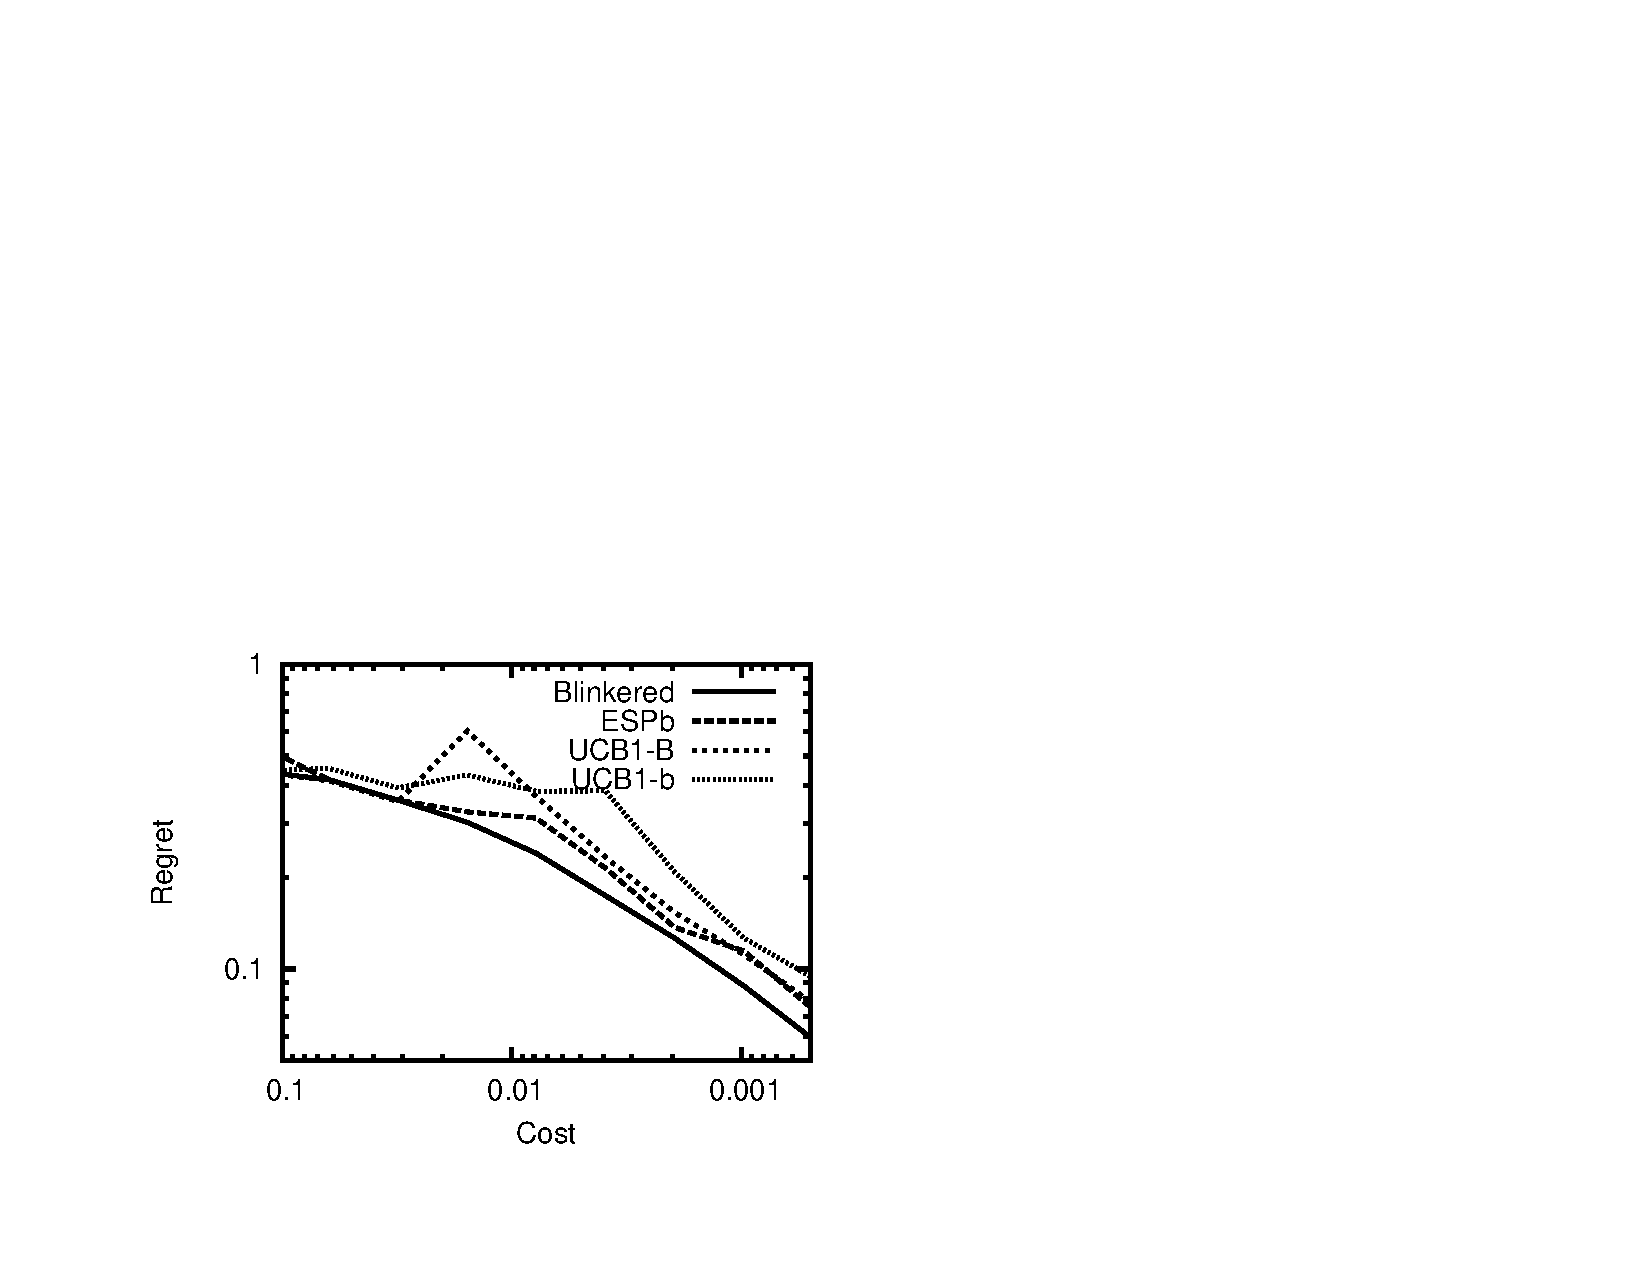
\includegraphics[scale=0.7, trim=90 70 400 300]{blinkered-regret.pdf}
\caption{Average regret of various policies as a function of the cost in 
a 25-action Bernoulli sampling problem.  Averaged over 1000 trials.}
\label{fig:blinkered}
\end{figure}

\begin{comment}
set xlabel "Cost"
set ylabel "Regret"

set terminal postscript enhanced linewidth 2
set output "blinkered-regret.ps"
set size 0.5, 0.5

set logscale xy

set key left bottom
plot [0.1:0.0005] [0.05:1] "blinkered-regret.dat" title "Blinkered" with lines lw 2, "myopic-regret.dat" title "Myopic" with lines lw 2, "espb-regret.dat" title "ESPb" with lines lw 2, "ucb-blinkered-regret.dat" title "UCB1-B" with lines lw 2, "ucb-blinkered-table-regret.dat" with lines lw 2 title "UCB1-b"
\end{comment}



%% \section{Regret bounds and approximate policies}

%% [[Regret models: simple regret, regret with cost per sampling; regret goes to zero as c does]]

%% [[Expected simple regret bounds for normal case?]]

%% [[Blinkered sampling]]

%% [[ESPb: Frazier's continuous time approximation]]

  

\section{Upper bounds on Value of Information}\label{approx-nonbayesian-section}

%% Solomon: Text presumably should be placed after the relevant theorems.

\begin{comment}
	Theorem \ref{thm:optimal-myopic} provides necessary conditions
	for a stopping condition for the optimal policy in terms of a myopic
	policy, but that does not preclude premature stopping of a greedy policy.
	Conversely, Theorem \ref{thm:myopic-optimal} provides sufficient conditions, but these 
	conditions are hard to evaluate in practice.

	The myopic selection policy uses
	the intrinsic value of information (VOI) $\Lambda_i$ of testing an arm~$i$, which is
	the expected reward of the best arm given the information obtained by the test,
	minus the expected reward of the best arm according to the current information state.
	Unfortunately, the pure \textit{myopic} VOI estimate is of little use in
	Monte-Carlo sampling, since the effect of a single sample is small,
	and the myopic VOI estimate will often be zero.

	Instead, we generalize myopic policies to include ``semi-myopic"
	up to $N$ samples of the same arm; these are called ``blinkered" policies.
	Such policies allow potentially unlimited lookahead, but only in a single ``direction'' (one specific arm),
	as if we ``had our blinkers on''.	
\end{comment}

%% Solomon: end text to be (possibly moved).

In many practical applications of the selection problem, such as search in
the game of Go, prior distributions are unavailable.\footnote{The analysis is also applicable to
some Bayesian settings, using ``fake" samples to simulate prior distributions.}
In such cases, one can still bound
the value of information of myopic policies using {\em concentration
inequalities} to derive distribution-independent bounds on the
VOI. We obtain such bounds under the
following assumptions:
\begin{enumerate}
\item Samples are iid given the value of the arms (variables), as in the Bayesian schemes such as Bernoulli
sampling.
\item The expectation of a selection in a belief state is equal to the sample mean (and therefore,
   after sampling terminates, the arm with the greatest sample mean will be selected).
\end{enumerate}

When considering possible samples in the blinkered semi-myopic setting,
two cases are possible: either
	the arm $\alpha$ with the highest sample mean $\overline
  	X_\alpha$ is tested, and $\overline X_\alpha$ becomes lower than
 	$\overline X_\beta$ of the second-best arm $\beta$;
or, 
	another arm~$i$ is tested, and $\overline X_i$ becomes higher
    than $\overline X_\alpha$.


Our bounds below are applicable to any bounded distribution (without loss of generality 
bounded in $[0,1]$). Similar
bounds can be derived for certain unbounded distributions, such as the
normally distributed prior value with normally distributed
sampling.
We derive a VOI bound for testing an arm a fixed $N$ times,
where $N$ can be the remaining budget of available samples or
any other integer quantity.
Denote by  $\Lambda_i^b$ the intrinsic VOI of testing the $i$th arm
$N$ times, and the number of
samples already taken from the $i$th arm by $n_i$.
\begin{thm} $\Lambda_i^b$ is bounded from above as
\begin{align}
\label{eqn:thm-be}
  \Lambda_\alpha^b&\le \frac {N \overline X_\beta^{n_\beta}} {n_\alpha} \Pr(\overline X_\alpha^{n_\alpha+N}\le\overline X_\beta^{n_\beta})\nonumber\\
\Lambda_{i|i\ne\alpha}^b&\le \frac {N(1-\overline X_\alpha^{n_\alpha})} {n_i}\Pr(\overline   X_i^{{n_i}+N}\ge\overline X_\alpha^{n_\alpha})
\end{align}
\label{thm:be}
\end{thm}
\begin{hiddenproof}
	\vspace{-2em}
	\begin{proof} For the case $i\ne \alpha$, the probability that the
	  $i$th arm is finally chosen instead of $\alpha$ is
	  $\Pr(\overline X_i^{n_i+N} \ge \overline X_\alpha^{n_\alpha})$. $X_i \le 1$,
	  therefore $\overline X_i^{n_i+N}\le \overline
	  X_\alpha^{n_\alpha}+\frac {N(1-\overline X_\alpha^{n_\alpha})} {N+n_i}$. Hence, the intrinsic value of blinkered
	  information is at most: 
	\begin{align}
	\label{eq:simplistic}
	\frac{ N(1-\overline  X_\alpha^{n_\alpha})}
	  {N+n_i}&\Pr(\overline X_i^{{n_i}+N}\hspace{-0.5em}\ge\overline X_\alpha^{n_\alpha})\nonumber \\
	&\le\frac{ N(1-\overline  X_\alpha^{n_\alpha})}
	{n_i}\Pr(\overline X_i^{{n_i}+N}\hspace{-0.5em}\ge\overline X_\alpha^{n_\alpha})
	\end{align}
	  Proof for the case $i=\alpha$ is similar.
	\end{proof}		
\end{hiddenproof}


The probabilities can be bounded from above using the
Hoeffding inequality \citep{Hoeffding.ineq}:
\begin{thm} The probabilities in \eqref{eqn:thm-be} are bounded from above as
\begin{align}
  \label{eqn:probound-blnk-hoeffding}
  \Pr&(\overline X_\alpha^{{n_\alpha}+N} \le \overline X_\beta^{n_\beta})
  \le 2\exp\left(- \varphi (\overline X_\alpha^{n_\alpha} - \overline X_\beta^{n_\beta})^2 n_\alpha
  \right)\nonumber\\
  \Pr&(\overline X_{i|i\ne\alpha}^{n_\alpha+N} \ge \overline X_\beta^{n_\beta})
  \le 2\exp\left(- \varphi (\overline X_\alpha^{n_\alpha} -\overline  X_i^{n_i})^2 n_i \right)
\end{align}
where $\varphi=\min \left(2(\frac {1+n/N} {1+\sqrt {n/N}})^2\right)=8(\sqrt 2 - 1)^2 > 1.37$.
\label{thm:hoeffding-prob-bounds}
\end{thm}


\begin{hiddenproof}
	\begin{proof}
	\eqref{eqn:probound-blnk-hoeffding}) follow from the
	observation that if $i\ne\alpha$, $\overline X_i^{n_i+N}>\overline X_\alpha^{n_i}$
	if and only if the mean $\overline X_i^N$ of $N$ samples from $n_i+1$
	to $n_i+N$ is at least $\overline X_\alpha^{n_i}+(\overline X_\alpha^{n_i}-\overline
	X_i^{n_i})\frac {n_i} N$.

	For any $\delta$, the probability that $\overline X_i^{n_i+N}$ is greater
	than $\overline X_\alpha^{n_i}$ is less than the probability that
	$\IE[X_i]\ge\overline X_i^n+\delta$
	\emph{or} $\overline X_i^N\ge \IE[X_i]+\overline X_\alpha^{n_\alpha}
	- \overline X_i^{n_i} - \delta +(\overline X_\alpha^{n_\alpha} - \overline X_i^{n_i})\frac {n_i} N$,
	thus, by the union bound, less than the sum of the probabilities:
	\begin{align}
	\Pr&(\overline X_i^{n_i+N}\ge \overline X_\alpha^{n_i})\nonumber\\
	   &\le\Pr(\IE[X_i]-\overline X_i^{n_i} \ge \delta)\\
	   &\hspace{0.25em}+\Pr\left(\overline X_i^N\hspace{-0.5em} - \IE[X_i] \ge \overline X_\alpha^{n_\alpha}\hspace{-0.5em}
	           - \overline X_i^{n_i}\hspace{-0.5em} - \delta +(\overline X_\alpha^{n_\alpha}\hspace{-0.5em} - \overline X_i^{n_i})\frac {n_i} N\right)\nonumber
	\end{align}
	Bounding the probabilities on the right-hand side using the Hoeffding
	inequality, obtain:
	\begin{align}
	\Pr&(\overline X_i^{n_i+N}\ge \overline X_\alpha^{n_\alpha})\le \nonumber\\
	    &\exp(-2\delta^2n_i)+\nonumber\\
	    &\quad\exp\left(-2\left((\overline X_\alpha^{n_\alpha}\hspace{-0.5em}
	         - \overline X_i^{n_i})\left(1+\frac {n_i} N\right)
	         - \delta\right)^2N\right)
	\label{eqn:app-hoeffding-le-maxexp}
	\end{align}
	Find $\delta$ for which the two terms on the right-hand side of
	\eqref{eqn:app-hoeffding-le-maxexp} are equal:
	\begin{equation}
	\exp(-\delta^2n) = \exp\left(-2\left((\overline X_\alpha - \overline X_i)(1+\frac {n_i} N) - \delta\right)^2N\right)\label{eqn:app-hoeffding-eq-exp}
	\end{equation}
	Solve \eqref{eqn:app-hoeffding-eq-exp} for $\delta$: $\delta=\frac {1+\frac {n_i} N} {1+\sqrt {\frac {n_i} N}} (\overline X_\alpha^{n_\alpha}\hspace{-0.5em}
	- \overline X_i^{n_i}) \ge 2(\sqrt 2 - 1)(\overline X_\alpha^{n_\alpha}\hspace{-0.5em}-\overline X_i^{n_i})$. Substitute $\delta$ into 
	\eqref{eqn:app-hoeffding-le-maxexp} and obtain
	\begin{align}
	\Pr&(\overline X_i^{n_i}\ge \overline X_\alpha^{n_\alpha}) \nonumber\\
	& \le 2\exp\left(-2\left( \frac {1+\frac {n_i} N} {1+\sqrt {\frac {n_i} N}}
	                          (\overline X_\alpha^{n_\alpha} - \overline X_i^{n_i})\right)^2 n_i\right)\nonumber \\
	& \le 2\exp(-8(\sqrt 2 - 1)^2(\overline X_\alpha^{n_\alpha} - \overline X_i^{n_i})^2n_i)\nonumber\\
	& = 2\exp(-\varphi(\overline X_\alpha^{n_\alpha} - \overline X_i^{n_i})^2n_i)
	\end{align}
	Derivation for the case $i=\alpha$ is similar.
	\end{proof}	
\end{hiddenproof}

\begin{crl}
An upper bound on the VOI estimate $\Lambda_i^b$ is obtained
by substituting \eqref{eqn:probound-blnk-hoeffding} into \eqref{eqn:thm-be}.
\begin{align}
  \label{eqn:bound-blnk-hoeffding}
  \Lambda&_\alpha^b \le \hat\Lambda_\alpha^b=\frac {2N\overline X_\beta^{n_\beta}} {n_\alpha}\exp\left(- \varphi(\overline X_\alpha^{n_\alpha}\hspace{-0.5em} - \overline X_\beta^{n_\beta})^2 n_\alpha\right)\nonumber\\
  \Lambda&_{i|i\ne\alpha}^b\le \hat\Lambda_i^b=  \frac {2N(1-\overline  X_\alpha^{n_\alpha})} {n_i}\exp\left(- \varphi(\overline X_\alpha^{n_\alpha}\hspace{-0.5em} - \overline X_i^{n_i})^2 n_i\right)
\end{align}
\label{crl:bound-blnk-hoeffding}
\end{crl}
\vspace{-2em}

More refined bounds can be obtained through tighter estimates on the
probabilities in \eqref{eqn:thm-be}, for example, based on the empirical Bernstein
inequality~\citep{MaurerPontil.benrstein}, or through a more careful
application of the Hoeffding inequality, resulting in:
\begin{align}
\Lambda_i^b&\le\frac {N\sqrt \pi} {n_i \sqrt {n_i}}
  \left[\mathrm{erf}\left((1\hspace{-0.25em}-\hspace{-0.25em}\overline X_i^{n_i})\sqrt {n_i}\right)
      \hspace{-0.25em}-\hspace{-0.25em}\mathrm{erf}\left((\overline X_\alpha^{n_\alpha}\hspace{-0.5em} - \overline X_i^{n_i})\sqrt{n_i}\right)\right]\nonumber\\
\Lambda_\alpha^b&\le\frac {N\sqrt \pi} {n_\alpha \sqrt {n_\alpha}}
  \left[\mathrm{erf}\left(\overline X_\alpha^{n_\alpha}\sqrt {n_\alpha}\right)
      -\mathrm{erf}\left((\overline X_\alpha^{n_\alpha}\hspace{-0.5em} - \overline X_\beta^{n_\beta})\sqrt{n_\alpha}\right)\right]
\label{eqn:erf-blinkered}
\end{align}



Selection problems usually separate out the decision of {\em whether} to
sample or to stop (called the stopping policy), and {\em what} to sample.
We'll examine the first issue here, along with the empirical evaluation 
of the above approximate algorithms, and the second in the following section.

Assuming that the sample costs are constant,
a semi-myopic policy will decide to test the arm that has the best
current VOI estimate. 
When the distributions are unknown, it makes sense
to use the upper bounds established in \thmref{thm:be}, as we do in the following.
This evaluation assumes a fixed budget of samples, which is
completely used up by each of the candidate schemes, making a stopping
criterion irrelevant.

\begin{figure}[h!]
\centering
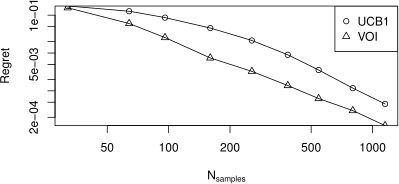
\includegraphics[scale=0.6]{flat.pdf}
\caption{Average regret of various policies as a function of the fixed number 
of samples in a 25-action Bernoulli sampling problem, over 10000 trials.}
\label{fig:random-instances}
\end{figure}

The sampling policies are compared on random Bernoulli
selection problem instances. \figref{fig:random-instances} shows results for
randomly-generated selection problems with 25 Bernoulli arms, where
the mean rewards of the arms are distributed uniformly in~$[0,1]$, 
for a range of sample budgets~$200..2000$, with multiplicative
step of~$2$, averaging over 10000 trials.  We compare UCB1 with the 
policies based on the bounds in
\eqref{eqn:bound-blnk-hoeffding} (VOI) and
\eqref{eqn:erf-blinkered} (VOI+).
UCB1 is always considerably worse than the VOI-aware sampling policies.





\section{Sampling in trees}
\label{sec:empirical-evaluation}\label{mcts-section}

The previous section addressed the selection problem in the flat case.
Selection in trees is more complicated.  The goal of Monte-Carlo tree 
search \citep{Chaslot.montecarlo} at the root node 
is usually to select an action that appears to be the best based on outcomes
of \textit{search rollouts}.
But the goal of rollouts at non-root nodes
is different than at the root: here it is important to better approximate the
value of the node, so that selection at the root can be more informed. The exact analysis
of sampling at internal nodes is outside the scope of this paper. At present we 
have no better proposal for internal nodes than to use UCT there.

We thus propose the following hybrid sampling scheme: 
	at the \emph{root node}, sample based on the VOI estimate;
	at \emph{non-root nodes}, sample using UCT.

Strictly speaking, even at the root node the stationarity assumptions\footnote{This is not a restriction,
however, of the general formalism in \secref{sec:optimal}.} 
underlying our belief-state
MDP for selection do not hold exactly. UCT is an adaptive scheme, and therefore the values
generated by sampling at non-root nodes will typically cause values observed at
children of the root node to be non-stationary. 
Nevertheless, sampling based on VOI estimates
computed as for stationary distributions works well in
practice. As illustrated
by the empirical evaluation (\secref{sec:empirical-evaluation}),
estimates based on upper bounds on the VOI result in good sampling
policies, which exhibit performance comparable to the performance of
some state-of-the-art heuristic algorithms.


\subsection{Stopping criterion}
\label{sec:control-stopping-criterion}

When a sample has a known cost commensurable with the value of
information of a measurement, an upper bound on the intrinsic VOI can also
be used to stop the sampling if the intrinsic VOI of any arm
is less than the total cost of sampling $C$:
\begin{equation}
\mbox{stop if } \max_i \Lambda_i \le C
\end{equation}
The VOI estimates of \eqrefs{eqn:thm-be}{eqn:bound-blnk-hoeffding} 
include the remaining sample budget $N$ as a
factor, but given the cost of a single sample $c$, the cost of the
remaining samples accounted for in estimating the intrinsic VOI is
$C=cN$. $N$ can be dropped on both sides of the inequality,
giving a reasonable stopping criterion:
\begin{align}
\frac 1 N \Lambda_\alpha^b \le&\frac {\overline X_\beta^{n_\beta}}
  {n_\alpha}\Pr(\overline X_\alpha^{n_\alpha+N}\le\overline
  X_\beta^{n_\alpha})\le c\nonumber\\
\frac 1 N \max_i\Lambda_i^b\le &\max_i\frac {(1-\overline X_\alpha^{n_\alpha})} {n_i}\Pr(\overline
  X_i^{n_i+N}\ge\overline X_\alpha^{n_\alpha})\le c\nonumber\\
    &\forall i: i\ne\alpha
\label{eqn:stopping-blnk}
\end{align}
The empirical evaluation (\secref{sec:empirical-evaluation})
confirms the viability of this stopping criterion and illustrates the
influence of the sample cost $c$ on the performance of
the sampling policy. When the sample cost $c$ is unknown, one can perform initial calibration experiments
to determine a reasonable value, as done in the following.

\subsection{Sample redistribution in trees}
\label{sec:control-redistribution}

The above hybrid approach assumes
that the information obtained from rollouts in the
current state is discarded after an real-world action is selected. In practice,
many successful Monte-Carlo tree search algorithms reuse rollouts
generated at earlier search states, if the sample traverses the
current search state during the rollout; thus, the value of information of a rollout is
determined not just by the influence on the choice of the action at
the current state, but also by its potential influence on the choice at future
search states.

One way to account for this reuse would be to incorporate the
`future' value of information into a VOI estimate. However, this 
approach requires a nontrivial extension of the theory of metareasoning for search.
Alternately, one can behave myopically with respect to the search tree depth:
\begin{enumerate}
\item Estimate VOI as though the information is discarded after each step,
\item Stop early if the VOI is below a certain threshold
   (see \secref{sec:control-stopping-criterion}), and
\item Save the unused sample budget for search in future states, such that
   if the nominal budget is $N$, and the unused budget in the last state
   is $N_u$, the search budget in the next state will be $N+N_u$.
\end{enumerate}
In this approach, the cost of a sample in the current state is the
VOI of increasing the budget of a future state by one sample.  It is
unclear whether this cost can be accurately estimated, but supposing
a fixed value for a given problem type and algorithm implementation
would work. Indeed, the empirical evaluation (\secref{sec:emp-go})
confirms that stopping and sample redistribution based on a learned
fixed cost  substantially improve the performance of the VOI-based
sampling policy in game tree search.


\subsection{Playing Go against UCT}
\label{sec:emp-go}

The hybrid policies were compared on the game Go, a search domain
in which UCT-based MCTS has been particularly successful
\citep{Gelly.mogo}. A modified version of Pachi \citep{Braudis.pachi}, a state of the art
Go program, was used for the experiments:
\begin{itemize}
\item The UCT engine of Pachi was extended with VOI-aware sampling
  policies at the first step. 
\item The stopping criterion for the VOI-aware policy was
  modified and based solely on the sample cost, specified as
  a constant parameter. The heuristic stopping criterion for the
  original UCT policy was left unchanged.
\item The time-allocation model based on the fixed number of samples
  was modified for \textit{both the original UCT policy and the VOI-aware
  policies} such that 
  \begin{itemize}
    \item The same number of samples is available to
      the agent at each step, independently of the number of pre-simulated
      games;  
    \item If samples were unused at the current step,
      they become available at the next step. 
  \end{itemize}
\end{itemize}
While the UCT engine is not the most powerful engine of Pachi, it is still a strong
player. On the other hand, additional features of more advanced
engines would obstruct the MCTS phenomena which are the subject of
the experiment.
\begin{figure}[h!]
\centering
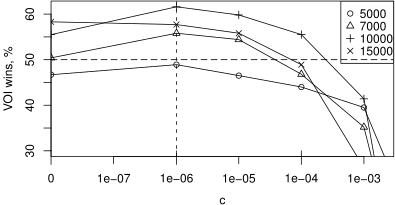
\includegraphics[scale=0.6]{uctvoi.pdf}
\caption{Winning rate of the VOI-aware policy in Go as a function of the cost $c$, for varying numbers of samples per ply.}
\label{fig:uctvoi}
\end{figure}
The engines were compared on the 9x9 board, for 5000, 7000, 1000, and
15000 samples (game simulations) per ply, each experiment repeated
1000 times. \figref{fig:uctvoi} depicts a calibration experiment,
showing the winning rate of the VOI-aware policy against UCT as a function of
the stopping threshold $c$ (if the maximum VOI of a sample is below
the threshold, the simulation is stopped, and a move is chosen). Each
curve in the figure corresponds to a certain number of samples per
ply.  For the stopping threshold of $10^{-6}$, the VOI-aware policy
is almost always better than UCT, and reaches the winning rate of
64\% for 10000 samples per ply.

\begin{figure}[h!]
\centering
\includegraphics[scale=0.6]{voi-wins.pdf}
\caption{Winning rate of the VOI-aware policy in Go as a function of the number of samples, fixing cost $c=10^{-6}$.}
\label{fig:voi-wins}
\end{figure}

\figref{fig:voi-wins}
shows the winning rate of VOI against UCT $c=10^{-6}$. In agreement with the intuition
(\figref{sec:control-redistribution}), VOI-based stopping and
sample redistribution is most influential for intermediate numbers of
samples per ply. When the maximum number of samples is too low, early
stopping would result in poorly selected moves. On the other hand,
when the maximum number of samples is sufficiently high, the VOI of
increasing the maximum number of samples in a future state is low.

Note that if we disallowed reuse of samples in both Pachi and
in our VOI-based scheme, the VOI based-scheme
win rate is even higher than shown in \figref{fig:voi-wins}. This is as expected,
as this setting (which is somewhat unfair to Pachi) is closer to
meeting the assumptions underlying the selection MDP.



\section{Conclusion}

The selection problem has numerous applications. This paper formalized the
problem as a belief-state MDP and proved some important properties of the 
resulting formalism. An application of the selection problem to control of
sampling was examined, and the insights provided by properties of the MDP 
led to approximate solutions that improve the state of the art. This was
shown in empirical evaluation both in ``flat" selection and when extending
the methods to game-tree search for the game of Go.

The methods proposed in the paper open up several new research
directions. The first is a better approximate solution of the MDP,
that should lead to even better flat sampling algorithms for
selection. A more ambitious goal is extending the formalism to
trees---in particular, achieving better sampling at non-root nodes,
for which the purpose of sampling differs from that at the root.



\bibliographystyle{abbrvnat}
\bibliography{refs}


\end{document}
